\documentclass[../mit-general-chemistry.tex]{subfiles}
\begin{document}

\chapter{Bonding}



{\em Chemical bonds} is an arrangement of electrons and nuclei of the
bonded atoms result in a lower energy than for the separate atoms.

\section{Covalent bonds}

A {\em covalent bond} results when a pair of electrons is shared
between two atoms.


\begin{example}
  The energy of two separate hydrogen atoms is
  \begin{equation*}
    E = 2 \cdot -1312~\si{\kilo\joule\per\mol} = -2624~\si{\kilo\joule\per\mol}
  \end{equation*}

  whereas a molecule of hydrogen gas, \ce{H2} is
  \begin{equation*}
    E = -3048~\si{\kilo\joule\per\mol}
  \end{equation*}

  It turns out that \ce{H2} is a lower state of energy for the two
  hydrogen atoms than \ce{2H} is.
\end{example}



When we are talking about bonds we are interested in bond strength,
the energy required to break the bond, as well as bond length.

We are also interested in internuclear distance ($r$). The distance
betwen two atomic nuclei in a molecule.


\begin{figure}[t]
  \begin{margincap}
    \begin{center}
      \includegraphics[width=.85\textwidth]{internucleardistance}
    \end{center}
    \caption{
      A {\em radial density function} (Schrodinger equation) over the
      $1s$ orbital of the hydrogen atom. Dynamic between coulomb
      forces result in an optimal intermolecular distance.
    }
  \end{margincap}
\end{figure}

The {\em dissociation energy}, \ded, the energy required to
break a bond (bond strength).

For the hydroge gas molecule
\begin{align*}
  \ded &= E_{\ce{2H}} - E_{\ce{H2}} =
  -2624~\si{\kilo\joule\per\mol} - (-3048~\si{\kilo\joule\per\mol}) =\\
  &= 424~\si{\kilo\joule\per\mol} \\
\end{align*}

We can thus conclude that the bond stength between the hydrogen atoms
in \ce{H2} is 424~\si{\kilo\joule\per\mol}.



When we draw plots over $\ded{r}$ it is common to  set the $\ded = 0$
for the energy of the two free hydrogen atoms and then we know what
the depth of the well in the diagram is from our previous
calculations ($\ded = 424~\si{\kilo\joule\per\mol}$).

Doing this we can also superimpose diagrams for other bonds and
compare bond strengths (graphically).











\section{Lewis structures}

Key to bonding: $e^-$ sharing to achieve a full valence shell.

Electrons are distributed in such a way that each element is
surrounded by eight electrons, an octet.

Each dot in a Lewis' structure represents a valence electron.

Lewis' structures are not based on quantum mechanics. His work was
what he observed far earlier than quantum mechanics.


\subsection{Octet rule}

Consider two fluorine atoms and their electrons

\hspace*{\fill}
\lewis{0.2:4:6:, F}
\hfill
\lewis{0:2:4.6:, F}
\hspace*{\fill}

When they are sharing one of their outermost $p$-electrons the octet
rule is satisfied and a covalent bond is formed.

\begin{center}
  \chemfig{\lewis{2:4:6:, F}-\lewis{0:2:6:, F}}
\end{center}

The straight line between the atoms in the figure above consists of the
two shared electrons.


The big exception to the octet rule is hydrogen (and helium) who's
most stable state is with two electrons and that is how it obtains a
full outer shell.

\begin{equation*}
  \lewis{0., H}\ +\ \lewis{0:2:4.6:, Cl} \ \rightarrow \chemfig{H-\lewis{0:2:6:, Cl}}
\end{equation*}

The chlorine atom has two bonding electrons and six lone pair
electrons (three pairs).


\subsection{Procedure for drawing Lewis' structures}


The MIT version

\begin{enumerate}
\item Draw a skeleton structure. H and F are always terminal
  atoms. The element with the lowest ionization energy goes in the
  middle (with some exceptions).

\item Count the total number of valence electrons, $v$. If there is a
  negative ion, add the absolute value of total charge to the count of
  valence electrons; if positive ion, subtract.

\item Count the total number of electrons needed for each atom to have a full
  valence shell, {\em octet rule}, $o$.

\item Subtract the number in step 2 (valence electrons) from the
  number in step 3 (total electrons for full shells). The result is
  the number of bonding electrons, $b = o - v$.

\item Assign 2 bonding electrons to each bond.

\item If bonding electrons remain, make some double or triple
  bonds. In general, double bonds form only between C, N, O, and
  S. Triple bonds are usually restricted to C, N, and O.

\item If valence electrons remain, assign them as lone pairs, giving
  octets to all atoms except hydrogen. Number of electrons to
  distribute over lone pairs can be calculated from $l = v - s$.

\item Determine the formal charge.
\end{enumerate}


\begin{remark}
  \begin{itemize}
  \item \ce{H} are allways terminal atoms
  \item \ce{O} is never in the middle
  \item methyl groups, \ce{CH3} are allways at the end
  \end{itemize}
\end{remark}




\begin{example}
  Draw a Lewis structure for \ce{CO2}.

  \begin{enumerate}
  \item Draw a sksleton structure. Omit bonds
    \ceeqstar{O C O}
  \item The total number of valence electrons $v = 2\times 6 + 4 =
    16$.
  \item There are three atoms, all from period 2 so $o = 3\times 8 = 24$.
  \item Number of electrons to share in bonds $b = 24 - 16 = 8$.
  \item Assign two electrons to each bond
    \begin{center}
      \chemfig{O-C-O}
    \end{center}
  \item We used four electrons of the eight bonding electrons so we
    have four left. We use them to form double bonds.
    \begin{center}
      \chemfig{O=C=O}
    \end{center}
  \item Now we have used all the bonding electrons. We still have $v -
    b = 16 - 8 = 8$ valence electrons left for lone pairs
    \begin{center}
      \chemfig{\lewis{2:6:,O}=C=\lewis{2:6:,O}}
    \end{center}
    This is the final Lewis structure.
  \end{enumerate}

  We have not learned how to calculate the formal charges within the
  molecule. That is next.
\end{example}


\subsubsection{The calculation of formal charge}

Formal charge is a measurement of the extent to which an atom has
gained or lost an electron, or actually a charge, in the process of
forming a covalent bond.


\begin{equation*}
  \formalcharge = V - L - \frac{S}{2}
\end{equation*}
where \formalcharge is the formal charge, $V$ is number of valence electrons,
$L$ lone pair electrons, $S$ shared electrons.

For an electronically-neutral molecule, the sum of the formal charges
for the individual atoms is (must be) zero.

For a molecule with a net charge of $c$ the sum of formal charges of
the individual atoms must be $c$.


We can use formal charges to compare the stability between Lewis'
structures. The most stable structure is the ones with lower absolute
values of formal charge.

We call the measurement $\sum |\formalcharge_i|$ the {\em charge
  separation} of the molecule.


\begin{example}
  The formal charge of \ce{CO2} is
  \begin{align*}
    \formalcharge_{\ce{O}} &= 6 - 4 - \frac{4}{2} = 0 \\
    \formalcharge_{\ce{C}} &= 4 - 0 - \frac{8}{2} = 0 \\
  \end{align*}

  Since $\sum |\formalcharge| = 0$ we consider \ce{CO2} a stable
  structure.
\end{example}


\paragraph{What if two structures have the same absolute value of formal charge?}

{\em Negative charge goes on the most electronegative atom}.

Consider \ce{CH3NHO-}. There are two resonance structures we can
draw. Doing so, we notice we can put the lonely hydrogen on either
the nitrogen or the oxygen atoms, either is fine.

\begin{center}
\schemestart
  $\left(~ \chemname{\chemfig{H-C(-[:-90]H)(-[:90]H)-\lewis{2:,N}(-[:270]H)-\chemabove{\lewis{0:2:6:,O}}{\raisebox{1.2mm}{\ensuremath{\ominus}}}}}{(a)} ~\right)^{-1}$
\arrow{<->}
  $\left(~ \chemname{\chemfig{H-C(-[:-90]H)(-[:90]H)-\chemabove{\lewis{2:6:,N}}{\raisebox{1.2mm}{\ensuremath{\ominus}}}-\lewis{2:6:,O}-H}}{(b)} ~\right)^{-1}$
\schemestop
\end{center}

The difference between (a) and (b) is that while (a) has a
\chemfig{N-H} bond, (b) has an \chemfig{O-H} bond. In term of formal
charges, none is more stable than the other. Instead we go to the rule
mentioned a few paragraphs up: {\em Negative charge goes on the most
  electronegative atom}. Looking up the electronegativity, for
instance in a periodic table, we find that
\begin{equation*}
  \chi_{\ce{C}} < \chi_{\ce{N}} < \chi_{\ce{O}} < \chi_{\ce{F}}
\end{equation*}

and since the negative \formalcharge is on the oxygen in (a) and on
nitrogen in (b), (a) is the lower energy/more stable structure.







\subsection{Resonance structures: ozone}

One single Lewis structure does not fully describe the electron
configuration of a molecule, instead we need to draw more Lewis
structures to describe that more appropriately.

We have

\begin{itemize}
\item three oxygen atoms
\item 18 valence electrons
\item to form three octets we need 24 electrons
\item this gives us six binding electrons
\end{itemize}

\begin{center}
\schemestart
  $\left(~ \chemname{\chemfig{\lewis{2:4:6:,O}-\lewis{2:,O}=\lewis{2:6:,O}}}{(a)} ~\right)$
\arrow{<->}
  $\left(~ \chemname{\chemfig{\lewis{2:6:,O}=\lewis{2:,O}-\lewis{0:2:6:,O}}}{(b)} ~\right)$
\schemestop
\end{center}

It turns out that these molecules are resonance structures \ce{O3} is
a blend of these two structures. The bonds are not a hundred percent
single and double bond, for instance and this is how we show it in
Lewis structures.

Resonance structures like these are also called resonance
hybrids. The true structure is a blend between (a) and (b).


Within resonance structures, electrons are delocalized, they are
shared between all three atoms. Electron pairs are shared over several
atoms, not just two.

Resonance structures are two (or more) structures with the same
arrangement of atoms, but a different arrangement of electrons.






\subsection{Exceptions to the octet rule}




\subsubsection{Case 1: Odd number of valence electrons}


It is not possible for every atom to have an octet because the octet
rule works by pairing electrons. If odd, one electron is left over.

Consider methyl, \ce{CH3}. Drawing the Lewis structure we have seven valence
electrons. We would need 14 electrons to fill all valence shells of
the atoms. This gives us 7 bonding electrons. Starting of with the
covalent bonds, we're left with one odd electron and we can't form a
bond with it. All three hydrogen atoms have full $1s$ shells, but the
carbon atom still needs two more electrons to fill the $2p$. That's
the empty spot and the carbon gets the odd electron.

\begin{center}
  \chemfig{H-\lewis{6.,C}(-[:90]H)-H}
\end{center}

This is a radical species. A molecule with an unpaired electron is
called a radical species or a free radical. Radicals are usually very
reactive, ``'cause they want to fill that octet''.

``Anti-oxidants get rid of free radicals'' in food and cosmetics (in
commercials).

\begin{example}[Free radicals in biology]
  Free radicals damage DNA. Being highly reactive, fre radicals react
  with DNA and break the strand of DNA. This is what happens in aging.

  We have a lot of free radicals in our bodies.

  We can insert them through cigarette smoke, which contains free
  radicals. Our bodies also produce free radicals in metabolism of
  food and oxygen.

  We have enzymes that repair damaged DNA and we also have
  anti-oxidants in our bodies.

  Brightly colored fruit are full of anti-oxidants and are full of
  chemicals that neutralize free radicals. A lot of
  vitamins also contain anti-oxidants, for example vitamin A and
  vitamin E.

  Free radicals are also essential for life. Some enzymes ``use'' free
  radicals to carry out essential reactions in the body. For example,
  RNRs catalyze an essential step in DNA synthesis and repair using
  free radicals.
\end{example}



Some radicals are more stable, like \ce{NO}, nitric oxide.

Nitrogen has five valence electrons, oxygen has six. We have eleven
altogether. We would need 16 to fill both valence shells. That leaves
us five bonding electrons. We form a double bond between the atoms,
put the odd binding electron on the nitrogen and distribute the rest
of the valence electrons among th atoms. We get the following Lewis
structure

\begin{center}
  \chemfig{\lewis{2.6:,N}=\lewis{2:6:,O}}
\end{center}

Calculating the formal charges  we see that $\formalcharge_{\ce{N}} =
5 - 3 - 2 = 0$ and $\formalcharge_{\ce{O}} = 6 - 4 - 2 = 0$. So it is
a fairly stable free radical.

If we had put the odd electron on the oxygen, we would have had
$\formalcharge_{\ce{N}}  = 1$ and $\formalcharge_{\ce{O}} = -1$. If we
had done this and discovered the split charge, we should have tried to
put the odd electron on the nitrogen.

Nitric oxide is a signaling substance in the body. It causes smooth
muscle tissues in the tunica media to relax, which is called
vasodilation. This causes increased blood flow.

Viagra inhibits breakdown of nitric oxide in the body which causes
increase in blood flow in parts of the body.



Now, consider \ce{O2}.

The Lewis structure is NOT (as the result from the standard procedure
would yield)

\begin{center}
  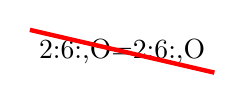
\begin{tikzpicture}
    \node{\chemfig{\lewis{2:6:,O}=\lewis{2:6:,O}}};
    \draw [red, ultra thick] (current bounding box.north west) -- (current bounding box.south east);
  \end{tikzpicture}
\end{center}

but  

\begin{center}
  \chemfig{\lewis{4.2:6:,O}-\lewis{0.2:6:,O}}
\end{center}

We have two radicals. In reality, \ce{O2} is a biradical. Finding
biradicals is not possible to discover using the Lewis structure
procedure. To predict this structure we need molecular orbital (MO)
theory which takes quantum mechanics into account (which Lewis
structures do not). This will come up in following chapters.









\subsubsection{Case 2: Octet deficient molecules}

Some molecules are stable with incomplete octet. This happens almost
exclusively with Group 13 elements, \ce{B}, \ce{Al} and so on. Be
aware when thos atoms are involved.

Consider \ce{BF3}, boron have three valence electrons, fluoride have
seven each. A total of 24. We need 32 electrons for full valence
shells so we need to share 8 electrons. That's three single bonds and
one double.

\begin{center}
  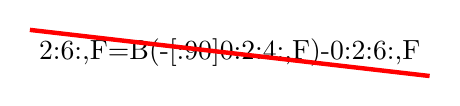
\begin{tikzpicture}
    \node{\chemfig{\lewis{2:6:,F}=B(-[:90]\lewis{0:2:4:,F})-\lewis{0:2:6:,F}}};
    \draw [red, ultra thick] (current bounding box.north west) -- (current bounding box.south east);
  \end{tikzpicture}
\end{center}

We get the formal charges
\begin{align*}
  \formalcharge_{\ce{B}} &= 3 - 0 - 4 = -1 \\
  \formalcharge_{\ce{F}\text{DB}} &= 7 - 4 - 2 = 1 \\
  \formalcharge_{\ce{F}} &= 7 - 6 - 1 = 0 \\
\end{align*}

which looks pretty good. But this is not the actual
structure. Experiments suggest that all three \chemfig{F-B} bonds are
of the same length, that of a single bond.

It turns out that

\begin{center}
  \chemfig{\lewis{4:2:6:,F}-B(-[:90]\lewis{0:2:4:,F})-\lewis{0:2:6:,F}}
\end{center}

yields $\formalcharge = 0$ for all four atoms and this is thus more
stable than the first structure. This is a good example of the
possible benefits of trying different solutions.

This structure shows the peculiarity with boron and aluminum, they are
happy with six instead of eight electrons around them.









\subsubsection{Case 3: Valence shell expansion}

This one is easy to miss.

Valence shell expansion can only occur with a central atom with a $n
\geq 3$. Elements with a $n \geq 3$ have empty $d$-orbitals, which
mean more than eight electrons can fit around the central atom.

Expanded shells are most common when the central atom is large and
bonded to small, electronegative atoms.


Consider \ce{PCl5}. We see that if phosphorus is going to bond to five
chlorine atoms, we have already broken our octet rule.

We have 40 valence electrons, The six atoms would need 48 electrons to
fill outer shells. We need to share eight bonding electrons.

This is a problem since we need ten electrons to form five
\chemfig{P-Cl} bonds. We go right ahead, though, and fill in that last
bond.

This leaves us with 30 lone pair electrons that we share among the
terminal atoms.

We end up with the following Lewis structure:

\begin{center}
  \chemfig{P%
    (-[:270]\lewis{0:4:6:,Cl})%
    (-[:198]\lewis{2:4:6:,Cl})%
    (-[:342]\lewis{0:2:6:,Cl})%
    (-[:54]\lewis{0:4:2:,Cl})%
    (-[:126]\lewis{0:4:2:,Cl})}
\end{center}

We calculate the formal charges of the atoms
\begin{align*}
  &\formalcharge_{\ce{P}} = 5 - 0 - 5 = 0 \\
  &\formalcharge_{\ce{Cl}} = 7 - 6 - 1 = 0  \\
\end{align*}

So this is a stable structure.

In this case  it was fairly obvious that we needed to add the extra
pair of bonding electrons since that was the only way to construct the
molecule.

Another case of valence shell expansion we see in \ce{CrO4^2-}. Doing
the Lewis structure, we see that we have $6 + 6\times 4 + 2 = 32$ valence
electrons. To fill the outer shells of all the atoms we would need 40
electrons so we need to share $40 -32 = 8$ binding electrons.

We get the Lewis structure

\begin{center}
  $\left[~
    \chemfig{\lewis{2:4:6:,O}-Cr(-[:90]\lewis{0:2:4:,O})(-[:270]\lewis{0:4:6:,O})-\lewis{0:2:6:,O}}
  ~\right]^{-2}$
\end{center}

The formal charges of the atoms are $\formalcharge_{\ce{Cr}} = 6 - 0 -
4 = 2$ and $\formalcharge_{\ce{O}} = 6 - 6 - 1 = -1$. We can check
this by using these figures to calculate the total charge $= 2 + 4
(-1) = -2$, which is the charge. This structure have some charge
separation and perhaps we can do better, in terms of stability.

It has been observed, experimentally, that the bonds of \ce{CrO4^2-}
are not single bonds but somewhere both bond length and strength is in
between that of single and double bonds.

The way we can illustrate wandering electrons is through resonance
structures.

\begin{center}
\schemestart
  $\left[~
    \chemfig{\lewis{2:6:,O}=Cr(-[:90]\lewis{0:2:4:,O})(-[:270]\lewis{0:4:6:,O})=\lewis{2:6:,O}}
  ~\right]^{-2}$
\arrow{<->}
$\cdots$
\arrow{<->}
  $\left[~
    \chemfig{\lewis{2:4:6:,O}-Cr(=[:90]\lewis{0:4:,O})(=[:270]\lewis{0:4:,O})-\lewis{0:2:6:,O}}
  ~\right]^{-2}$
\schemestop
\end{center}

There are actually six resonance structures for this molecule, with
all the different combinations of double bond position.

The formal charges in tese structures are $\formalcharge_{\ce{Cr}} = 6
- 0 - 6 = 0$, $\formalcharge_{\ce{O}\text{-DB}} = 6 - 4 - 2 = 0$ and
$\formalcharge_{\ce{O}} = 6 - 6 - 1 = -1$.

In this structure there is less formal charge separation than in the
previous one. That is what we are looking for. That means a more
stable molecule. Note that the \ce{Cr}-atom has ten electrons in the
valence shell, which makes this a case of valence shell expansion. The
way we discovered it this time was through knowledge of experimental
observations.

\begin{remark}
  A {\em resonance structure} is a structure where all the atoms
  remain in place, but the electrons move around.

  Formal charges are the same for different resonance structures so
  you only have to calculate the charges for one of them.
\end{remark}

Any time you can have an expanded octet, an expanded valence shell,
where you have $n \geq 3$, and if you with expanding valence shell you
lower the charge separation, you want to do that.







\subsection{Ionic bond}


Ionic bonds involve the complete transfer of one or many electrons
between two atoms. Bonding results from the electrostatic attraction
(coulomb force) between the cation and the anion.

\begin{remark}
  Whereas the keyword for covalent bonds is {\em sharing}, the keyword
  for ionic bonds is {\em transfer}.
\end{remark}

Formation of \ce{NaCl} from neutral \ce{Na} and \ce{Cl}. In forming
ionic compounds from neutral atoms, we need to think about the
ionization energy of the element the will for the cation and the
electron affinity of the element that is forming the anion. The sign
of the differences of those energies will tell us if this is a
reaction that will occur spontaneously or not.
\begin{align*}
  \ce{Na(g) &-> Na+(g) + e-} & \deltaE = \ionizationenergy = \SI{494}{\kilo\joule\per\mol} \\
  \ce{Cl(g) + e- &-> Cl-(g)} & \deltaE = -\electronaffinity = \SI{-349}{\kilo\joule\per\mol} \\
\end{align*}
So it costs \SI{494}{\kilo\joule} to create one mole of \ce{Na+} from
neutral \ce{Na} and \SI{349}{\kilo\joule} is released when one mole of
\ce{Cl-} is produced from \ce{Cl(g)}. If we sum up
\begin{align*}
  &\ce{Na(g) + Cl(g) -> Na+(g) + Cl-(g)} & \Delta E =
  \SI{+145}{\kilo\joule\per\mol} \\
\end{align*}
The formation of the ions from the neutral atoms has a positive
\deltaE which means the reactions cost energy and is thus not
favourable. What is favourable is when we get energy out and the
systems energy get lower, but what we see here is that we need to put
in energy in our system and another way of saying this is that the
process requires energy.

So where does this energy come from? The answer is {\em coulomb
  attraction}. There is one more force that we need to talk about
and that is the \deltaE of the formation of the \ce{NaCl}
\begin{equation*}
  \ce{Na+(g) + Cl-(g) -> NaCl(g)} \qquad \deltaE = \SI{-589}{\kilo\joule\per\mol} \\
\end{equation*}

So that is a huge negative number (release of energy) in this context.

Now we can add up the net energy change
\begin{align*}
  &\ce{Na(g) + Cl(g) -> NaCl(g)} & \deltaE = \SI{-444}{\kilo\joule\per\mol} \\
\end{align*}

The formation of \ce{NaCl} involves a net decrease in energy which
means that the reaction is favourable and will occur spontaneously.




\paragraph{Calculating the coulomb potential for a known $r$}
This way we can calculate an approximation of the strength of the
ionic bond which is the negative of the dissociation energy.
\begin{equation*}
  U(r) = \frac{z_!z_2e^2}{4\pi\epsilon_0r}
\end{equation*}
where $z_n$ is the charge of the ions, $e$ is the absolute value of
the charge of one electron, $\frac{1}{4\pi\epsilon_0} = k_e =
\SI{8.98755d9}{\newton\square\meter\per\square\coulomb}$ is Coulomb's
constant and $r$ is the bond length between the ions. For \ce{NaCl}
the bond length, $r = \SI{2.36}{\angstrom} =
\SI{2.36d-10}{\meter}$. We get

\begin{equation*}
  U(r) = \frac{(-1)(1)(1.602\times 10^{-19}\si{\coulomb})^2}{4\pi\epsilon_0\cdot\SI{2.36d-10}{\meter}} 
  = \SI{-9.774d-19}{\joule}
\end{equation*}

Now, this isn't the number we got before, but we want the number in
\si{\kilo\joule\per\mol} so we calculate

\begin{equation*}
  U(r) = \SI{-9.774d-19}{\joule} \times \frac{\si{\kilo\joule}}{1000
    \si{\joule}} \times \frac{\num{6.023d23}}{\si{\joule}} = \SI{-589}{\kilo\joule\per\mol}
\end{equation*}

Which is the attractive force between the ions. The negative force
means it is an attraction.



\begin{remark}
  \dissociationenergy is the {\em dissociation energy}. It is the
  strength of a bond. What would it take to break that bond?
\end{remark}




\paragraph{Verification through experiments}
Above we calculated the net $\Delta E$ using \ionizationenergy of
\ce{Na} and \electronaffinity of \ce{Cl}. The calculated $\Delta E$ we
got was \SI{-444}{\kilo\joule\per\mol}.

Now, experiments have shown that this is not exactly the true
value. The experimentally found value of the \chemfig{Na-Cl} ionic
bond is a bit higher/weaker, it is \SI{-411}{\kilo\joule\per\mol}.

It is not strange that we got different values. The simple ionic model
only do basic assumptions. In reality the system is more complex.

\begin{center}
  \begin{tabular}{ll}
    Simple ionic model predicts:
    & $\Delta E = \SI{-444}{\kilo\joule\per\mol}$ \\
    & $\Delta E_d = \SI{444}{\kilo\joule\per\mol}$ \\
    \\
    Experiments measure:
    & $\Delta E = \SI{-411}{\kilo\joule\per\mol}$ \\
    & $\Delta E_d = \SI{411}{\kilo\joule\per\mol}$ \\
  \end{tabular}
\end{center}



We made the following assumptions
\begin{itemize}
\item Ignored repulsive interactions between ions of the same species
  (or same-sign charge). This results in a larger
  \dissociationenergy than experimental value.
\item We treated \ce{Na+} and \ce{Cl-} as point charges. This ignores
  quantum mechanics model of the atom, which introduces errors in
  calculations.
\end{itemize}

















\subsection{Polar covalent bond}

A {\em polar covalent bond} is formed by {\em unequal} sharing of
electrons between two atoms with different electronegativities.

In general, we consider a bond between two atoms where \[0.4 <
\Delta\chi < 1.7\qquad{\text{(Pauling scale)}}\] to be a polar bond.

\hspace*{\fill}
\chemfig{H-Cl}
\hfill
$\chi_{\ce{H}} = 2.2$
\hfill
$\chi_{\ce{Cl}} = 3.2$
\hspace*{\fill}


An electronegative atom (\ce{Cl} above) pulls the electron density
cloud towards itself. Which give it (a little bit of) a negative
charge while the other (\ce{H} above) is left with (a little bit of) a
positive charge. These charges are called partial charges and we use a
$\delta -$ or $\delta +$ to denote those charges.

\begin{center}
  \chemfig{\chemabove{H}{\scriptstyle\delta +}-\chemabove{Cl}{\scriptstyle\delta -}}
\end{center}


\paragraph{Dipole moment, $\vec{\mu}$}

Asymmetric charge distribution results in an electric dipole.

\begin{center}
  \begin{tikzpicture}
    \node[circle, draw, fill=green!20, radius=.5ex]
         [label={[label distance=1ex]90:$\delta+$}](a){A}; 
         \node [circle, draw, fill=green!20, right=of a, radius=.75ex] 
               [label={[label distance=1ex]90:$\delta-$}](b) {B};
         \draw[thick] (a) -- (b) node[midway, above] {$r$};
    \coordinate[below=1.5ex of a] (a1);
    \coordinate[below=1.5ex of b] (b1);
    \draw[ultra thick, ->] (a1) -- (b1)
    node[midway, below]{$\vec{\mu}$};
    \draw[ultra thick] ($ (a1) +(2mm, 2mm) $) -- ($ (a1) +(2mm, -2mm) $);
  \end{tikzpicture}
\end{center}

Magnitude of charge
\begin{equation*}
  \vec{\mu} = Q \cdot \vec{r}
\end{equation*}

Separation where $Q = |\delta e|$.

Dipole moments are measured in coulomb$\cdot$meters,
\si{\coulomb\meter}, or in debye
\begin{equation*}
  1~\text{debye} = 1~\si{\debye} = \SI{3.336d-30}{\coulomb\meter}
\end{equation*}


\subsubsection{Polar molecules}

Polar molecules have a non-zero net dipole moment.

We consider a covalent bond polar if the difference in
electronegativity between the atoms larger than $0.5$ (Pauling
scale).


Consider \ce{CO2}, which is a linear molecule. The electronegativity
of carbon (2.5) and oxygen (3.4) suggests that the \chemfig{C-O} bonds
are polar. If we draw the dipole moments we see that we have two equal
but opposite vectors pointing from the carbon towards the two oxygen
atoms. The two moments cancel each other out and \ce{CO2} is thus not
polar.

\begin{center}
  \chemfig{\lewis{2:6:,O}=C=\lewis{2:6:,O}}
\end{center}


In contrast, the \ce{H2O} has a bent shape due to the two free
electron pairs and also have a $\Delta\chi = 1.3$ which makes the
\chemfig{O-H} bonds polar. The bent shape makes the two polar dipole
moments work in an angle and they do not cancel each other out. This
makes the entire molecule polar and this gives water some of the
properties, characteristic of water.

\begin{center}
  \chemfig{\lewis{1:3:,O}(-[:218]H)(-[:322]H)}
\end{center}



In large organic molecules and in biomolecules, such as proteins, we
often consider the number of polar groups within the molecule. This
will tell us about whether the molecules are water soluble and how the
will fold.


Comparing vitamin A and vitamin B9 (folic acid) and counting the number
of polar covalent bonds in the molecules can give us an idea of why B9
is water soluble and vitamin A is not. The number of polar bonds in
the molecule tells us this.






\addsec{Summary}
\end{document}
